%%
%  ******************************************************************************
%  * #file    Szablon_raportu_EN_Latex.tex
%  * #author  Adrian Wójcik   adrian.wojcik(at)put.poznan.pl
%  *          
%  * #commit  Patryk Kościk   koscikpatryk(at)gmail.com
%  *          Modified the template for Projekt przejsciowy purposes          
%  *          
%  *
%  * #commit  Patryk Kościk   koscikpatryk(at)gmail.com
%  *          Zupełnie przewrócono na łeb formatke po taktycznym wyjasnieniu          
%  *          
%  * #version 1.1
%  * #date    09-Mar-2022
%  * #brief   PROJPRZEJ
%  *
%  ******************************************************************************
%%  
\documentclass[11pt, a4paper]{article}

\usepackage{SM_template}

% Wypełnijcie te dyrektywy zgodnie z waszym tematem
%
% \lab      -> NAZWA CZUJNIKA,          np.: 'DHT22'
% \comment  -> Króciutki opis co to,    np.: 'Cyfrowy czujnik temperatury'
% \author   -> Autor dokumentu          np.: Patryk Kościk
%
% Pamiętajcie o zmianie ścieżki w \addbibresourcue (!)

\lab{GY-Bm280}
\comment{Moduł cyfrowego czujnika ciśnienia i temperatury firmy Bosch}
\author{Dawid Sobczak}
\addbibresource{bib/GY-BM280.bib}
%
% Początek dokumentu
%
\begin{document}

%
% Strona tytułowa
%
\mainpage{GY-BM280/GY-BM280_photo}
\newpage

\section*{Opis elementu}
Elementem pomiarowym modułu jest piezorezystancyjny czujnik ciśnienia, charakteryzujący się wysoką odpornością EMC, wysoką dokładnością, liniowością oraz długoterminową stabilnością. BMP280 mieści się w niezwykle kompaktowej, 8-stykowej metalowej pokrywie LGA. Sensor operuje na niższych zakłóceniach, wspiera najnowsze metody filtracji oraz komunikację poprzez interfejs SPI. \\\\
Zasada działania modułu opiera się na piezorezystancyjnym czujniku ciśnienia oraz wyspecjalizowanym układzie scalonym ASIC. ASIC odpowiada za konwersję A/D oraz dostarcza wyniki tej konwersji poprzez interfejs cyfrowy.  Więcej informacji można znaleźć w nocie katalogowej dostępnej w \cite{bmp280_datasheet}.
%%%%%%%%%%%%%%%%%%%%%%%%%  TWO IMAGES SIDE BY SIDE  %%%%%%%%%%%%%%%%%%%%%%%%%%%%%
\vspace{0.25cm}
\begin{figure}[h]
\centering
%%%%%%%%%%%%%%%%%%%%%%%%%%%%%%%%%%%%%%%%%%%%%%%%%%%%%%%%%%%%%%%%%%%%%%%%%%%%%%%%%
\begin{subfigure}{.5\textwidth}
\centering
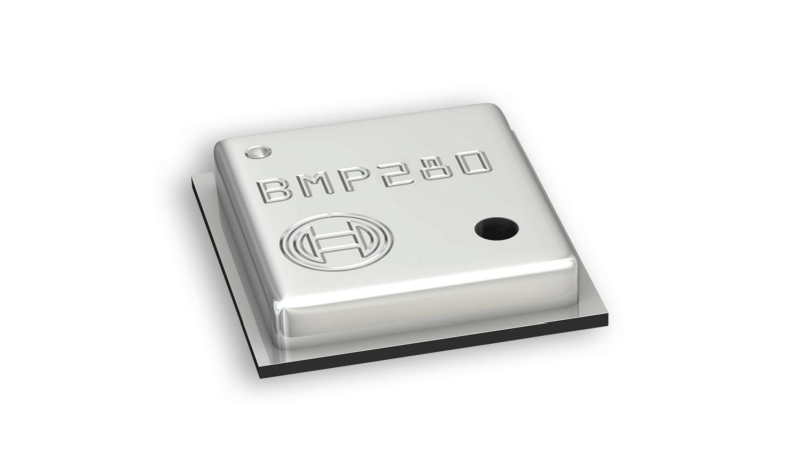
\includegraphics[width=\linewidth]{fig/GY-BM280/bmp280_photo.PNG}
\caption{Bosch BMP280 - zdjęcie}
\label{fig:_zdjecie_elementu}
\end{subfigure}%
%%%%%%%%%%%%%%%%%%%%%%%%%%%%%%%%%%%%%%%%%%%%%%%%%%%%%%%%%%%%%%%%%%%%%%%%%%%%%%%%%
\begin{subfigure}{.5\textwidth}
\centering
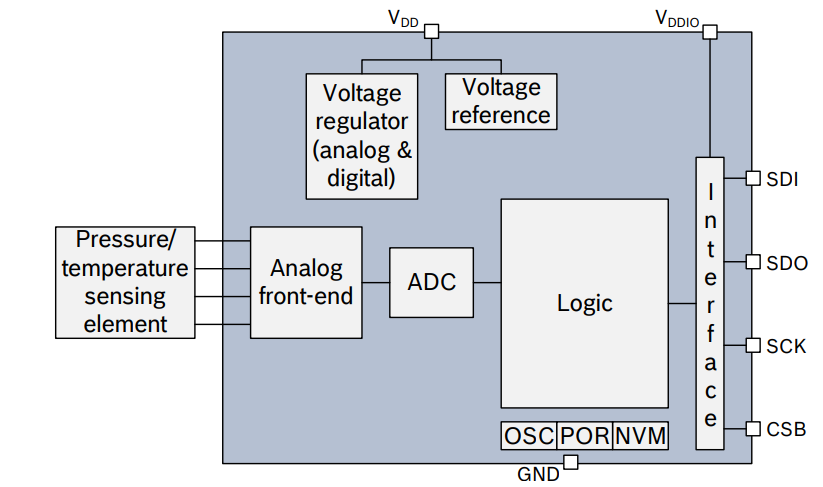
\includegraphics[width=\linewidth]{fig/GY-BM280/bmp280_diagram.PNG}
\caption{\centering Diagram blokowy modułu sensora BMP280}
\label{fig:_zasada_dzialania_elementu}
\end{subfigure}
%%%%%%%%%%%%%%%%%%%%%%%%%%%%%%%%%%%%%%%%%%%%%%%%%%%%%%%%%%%%%%%%%%%%%%%%%%%%%%%%%
% \caption{PODPIS}
\label{fig:element}
\end{figure}
\vspace{0.25cm}
%%%%%%%%%%%%%%%%%%%%%%%%%  TWO IMAGES SIDE BY SIDE  %%%%%%%%%%%%%%%%%%%%%%%%%%%%%
% \subsection{Opis modułu} REPLACE SUBSECTION WITH 1CM VSPACE
\vspace{0.75cm}
%%%%%%%%%%%%%%%%%%%%%%%%%  TWO IMAGES SIDE BY SIDE  %%%%%%%%%%%%%%%%%%%%%%%%%%%%%
\begin{figure}[h]
\centering
%%%%%%%%%%%%%%%%%%%%%%%%%%%%%%%%%%%%%%%%%%%%%%%%%%%%%%%%%%%%%%%%%%%%%%%%%%%%%%%%%
\begin{subfigure}{.5\textwidth}
\centering
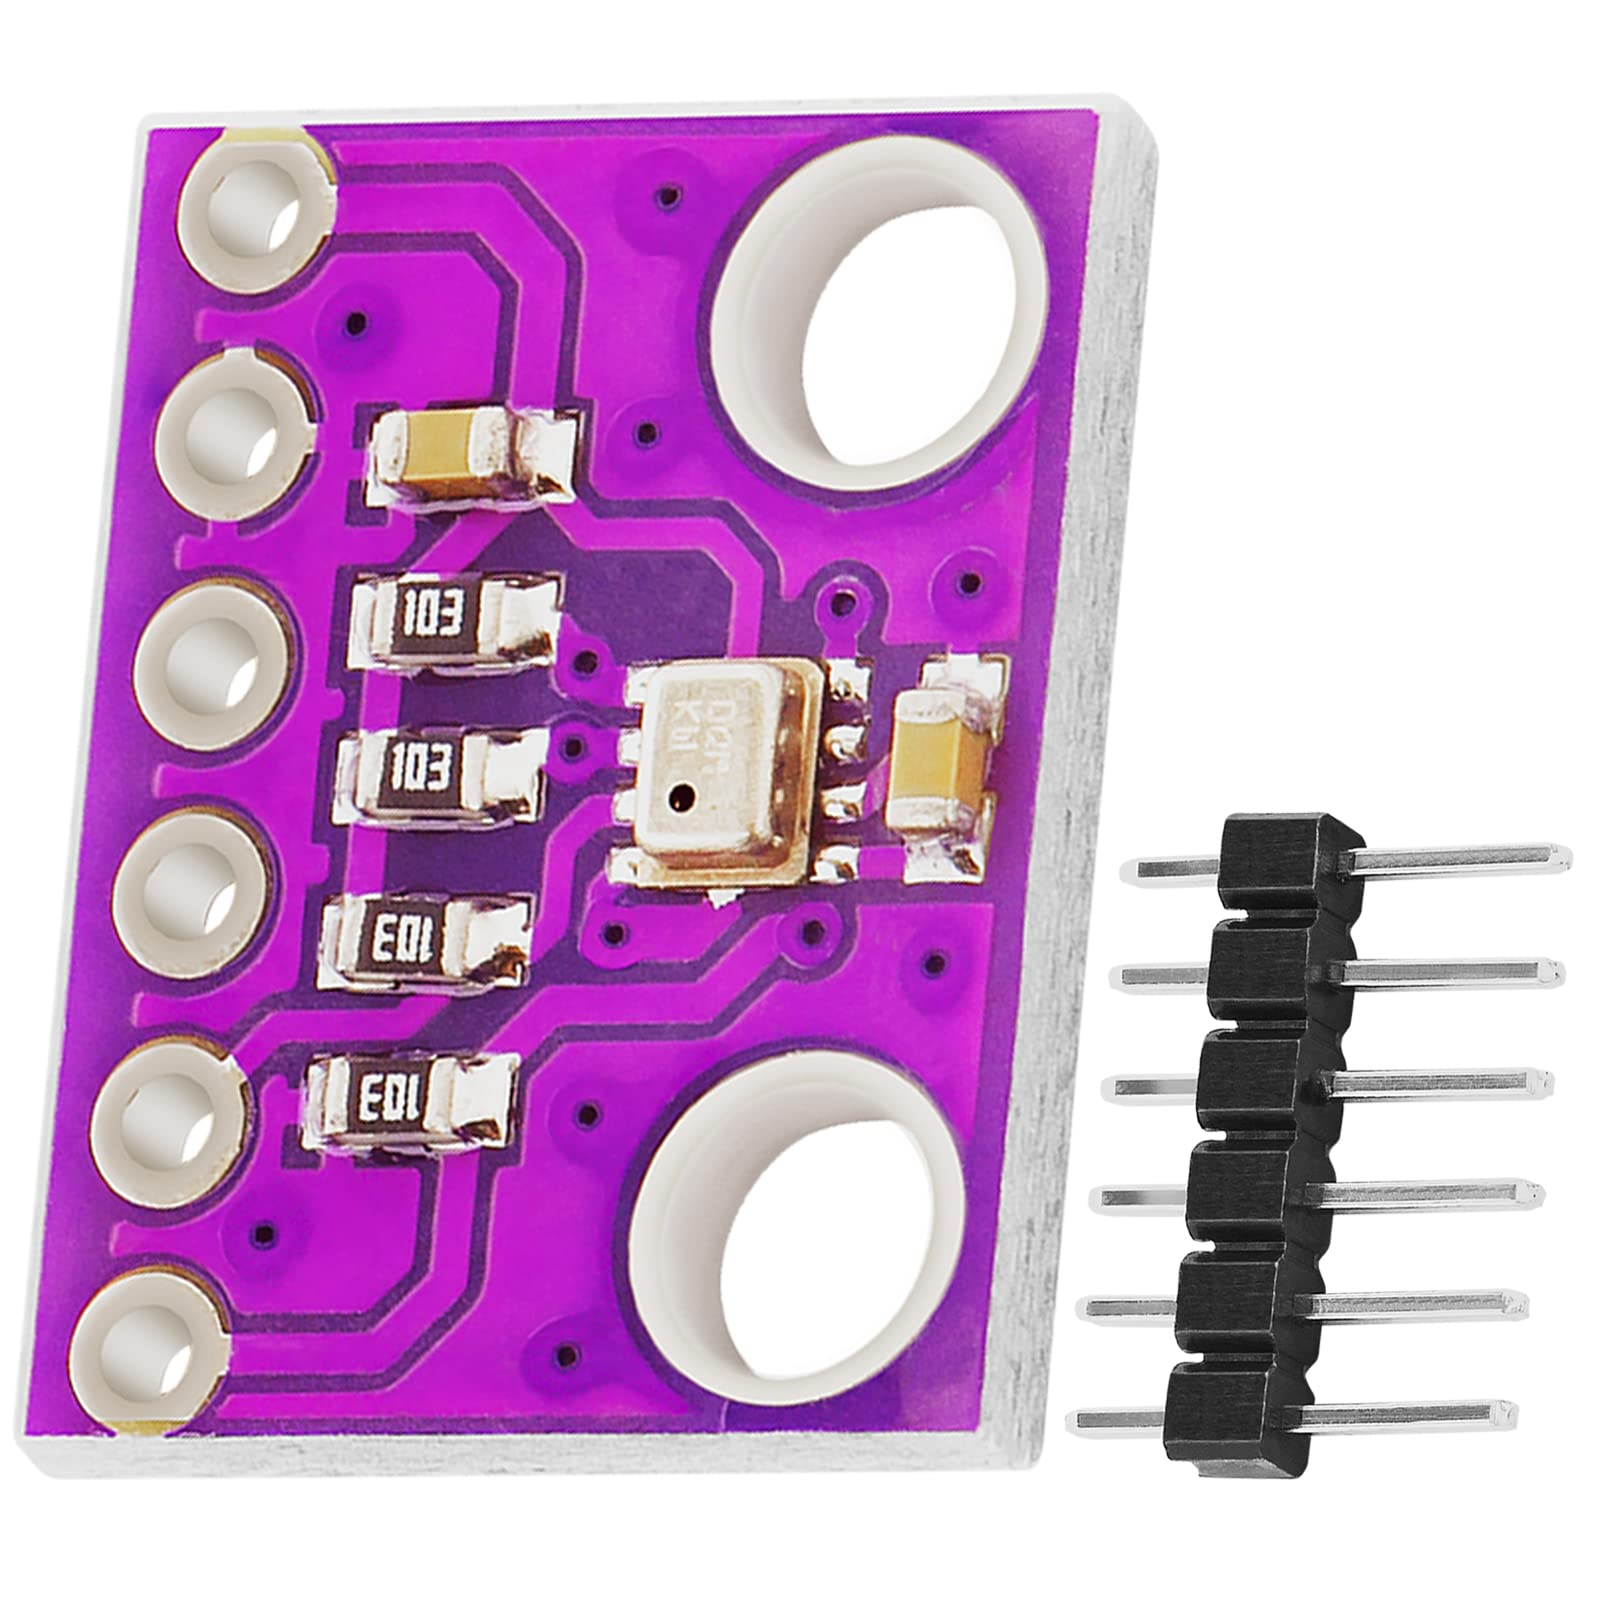
\includegraphics[width=.7\linewidth]{fig/GY-BM280/gy-bm280_photo_2.jpg}
\caption{Moduł GY-BM280 - zdjęcie \cite{Amazon:Zdjęcie}}
\label{fig:_zdjecie_modulu}
\end{subfigure}%
%%%%%%%%%%%%%%%%%%%%%%%%%%%%%%%%%%%%%%%%%%%%%%%%%%%%%%%%%%%%%%%%%%%%%%%%%%%%%%%%%
\begin{subfigure}{.5\textwidth}
\centering
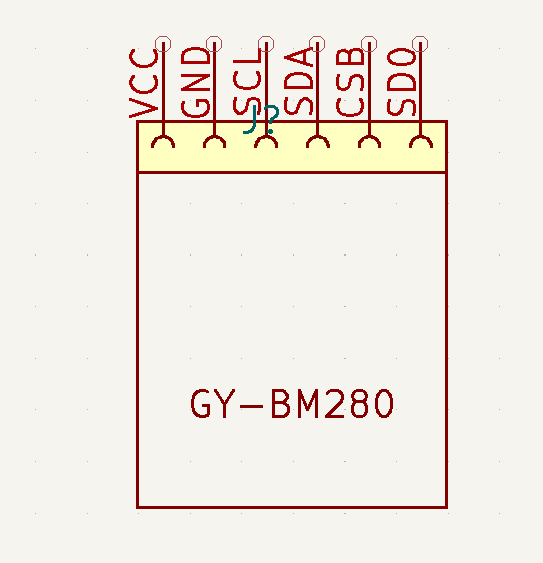
\includegraphics[width=.7\linewidth]{fig/GY-BM280/wyprowadzenia.PNG}
\caption{Wyprowadzenie modułu - schemat}
\label{fig:_schemat_modulu}
\end{subfigure}
%%%%%%%%%%%%%%%%%%%%%%%%%%%%%%%%%%%%%%%%%%%%%%%%%%%%%%%%%%%%%%%%%%%%%%%%%%%%%%%%%
\label{fig:modul}
\end{figure}
\vspace{0.5cm}
%%%%%%%%%%%%%%%%%%%%%%%%%  TWO IMAGES SIDE BY SIDE  %%%%%%%%%%%%%%%%%%%%%%%%%%%%%

\vspace{0.5cm}
Moduł GY-BM280 to specjalna plytka PCB, która zapewnia możliwość bezpośredniego podłączenia modułu do mikrokontrolera, bez konieczności prototypowania rezystorów typu pull-up/pull-down czy kondensatorów filtrujących. Moduł to gotowy element do aplikacji, wymaga zasilania napięciem od $1.6$ do $3.3$ [V].
\newpage
\begin{figure}[h]
    \centering
    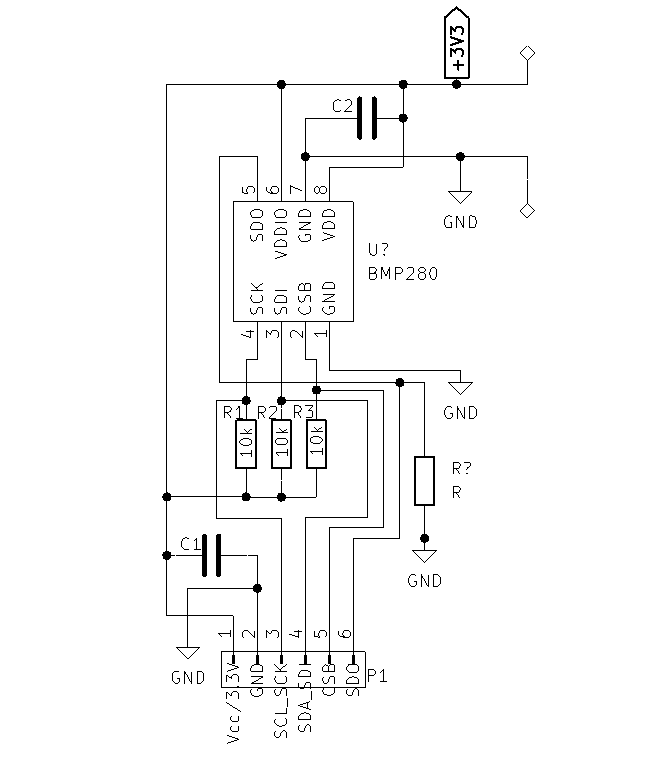
\includegraphics[width=0.8\textwidth]{fig/GY-BM280/modul_schemat_elektryczny.PNG}
    \caption{Kompletny schemat elektryczny modułu GY-BM280}
    \label{fig:polaczenie_ukladu}
\end{figure}
\newpage
\section{Użycie modułu}
\subsection{Mikrokontroler}
Aplikacja modułu wymaga połączenie mikrokontrolera z modułem w sposób opisany w tabeli (\ref{tab:tab1}) znajdującej się poniżej.
W tym przykładzie wykorzystywana jest komunikacja poprzez magistralę $I^2C$, dlatego konieczne jest wcześniejsza konfiguracja komunikacji na mikrokontrolerze. 

\vspace{0.5cm}
\begin{table}[h!]
    \centering
    \begin{tabular}{|c|c|c|c|} 
        \hline
        \multicolumn{2}{|c|}{NUCELO-F746ZG} & \multicolumn{2}{c|}{Moduł GY-BM280}  \\ 
        \hline
        Etykieta    &   Port i numer pinu   &   Nr pinu &   Etykieta    \\ \hline
        +3V3    &   -   &   1   &   VCC \\  \hline
        GND     &   -   &   2   &   GND \\  \hline
        PB9     &   D14 &   3   &   SCL \\  \hline
        PB6     &   D26 &   4   &   SDA \\  \hline
        N.C.    &   -   &   5   &   CSB \\  \hline
        N.C     &   -   &   6   &   SD0 \\  \hline
    \end{tabular}
    \caption{Połącznie pomiędzy modułem i mikrokontrolerem}
    \label{tab:tab1}
\end{table}

Dodatkowe schematy połączeń i konfiguracja mikrokontrolera oraz kod źródłowy wykorzystany w implementacji zostały
opisane w sekcji \texttt{Suplement \#1}.

\begin{figure}[h]
    \centering
    \includegraphics[width=0.8\textwidth]{fig/GY-BM280/1657055010846.jpg}
    \caption{Połączenie układu - zdjęcie}
    \label{fig:polaczenie_ukladu}
\end{figure}
\vspace{0.5cm}
Działanie modułu z w aplikacji z mikrokontrolerem zostało zaprezentowane na materiałe wideo zawartym w \texttt{\cite{yt1}}.

\newpage
\printbibliography[heading=bibintoc]

\end{document}